\providecommand{\qcor}[1]{\ulcorner#1\urcorner}   %
\providecommand{\cellpair}[5]{$\vcenter{\hbox{\begin{tikzpicture}[x=1.15em,y=1.15em]%
\node (s) at (0,0) {$#1$};%
\node (t) at (4.2,0) {$#2$};%
\draw[->] (0.75,0.32) to[bend left=18] (3.45,0.32);%
\node at (2.1,0.88) {$\scriptstyle#3$};%
\draw[->] (0.75,-0.32) to[bend right=18] (3.45,-0.32);%
\node at (2.1,-0.93) {$\scriptstyle#4$};%
\draw[->] (1.95,0.2) to[bend right=32] (1.95,-0.2);%
\node at (2.85,0) {$\scriptstyle#5$};%
\end{tikzpicture}}}$\ignorespaces}
\providecommand{\bijarrow}{\twoheadleftarrow\!\!\twoheadrightarrow}

\section{笛卡尔纤维化的可表示性}\label{sec:representability-of-cartesian-fibrations}

本节考虑与\trInfinityCosmos{}中\trInfinityCategory{}之间的一条\trIsofibration{}%
$p\colon E\twoheadrightarrow B$ 相关联的拟范畴\trIsofibration{}族
$p_{*}\colon\mathrm{Fun}(X,E)\twoheadrightarrow\mathrm{Fun}(X,B)$。我们的目标是%
证明：\trCartesianFibration、笛卡尔函子与\trDiscreteCartesianFibration{}这几个概念各自都在各种%
意义下是可表示地定义的：

\begin{proposition}\label{prop:discrete-cartesian-representable}
\trInfinityCosmos{} $\mathcal{K}$ 中的一条\trIsofibration{}
$p\colon E\twoheadrightarrow B$ 定义一条\trDiscreteCartesianFibration，当且仅当对所有的
$X\in\mathcal{K}$，$p_{*}\colon\mathrm{Fun}(X,E)\twoheadrightarrow\mathrm{Fun}(X,B)$
定义一条\trQuasiCategory{}的\trDiscreteCartesianFibration。
\end{proposition}

\begin{proof}
由于∞-宇宙中的\trEquivalence{}与单纯极限都是可表示地定义的概念，这立即由命题
5.5.8 给出的\trDiscreteCartesianFibration{}的刻画得到。
\end{proof}

\trCartesianFibration{}的可表示性则更为微妙：

\begin{proposition}\label{prop:cartesian-representable}
设 $p\colon E\twoheadrightarrow B$ 为\trInfinityCosmos{} $\mathcal{K}$ 中%
\trInfinityCategory{}之间的一条\trIsofibration。则 $p$ 是一条\trCartesianFibration，
当且仅当：
\begin{enumerate}[label=(\roman*)]
\item 对所有的 $X\in\mathcal{K}$，\trIsofibration{}
$p_{*}\colon\mathrm{Fun}(X,E)\twoheadrightarrow\mathrm{Fun}(X,B)$ 是%
\trQuasiCategory{}之间的一条\trCartesianFibration。
\item 对所有的 $f\colon Y\to X\in\mathcal{K}$，由诸限制映射定义的方块是一个%
笛卡尔函子：
\begin{center}
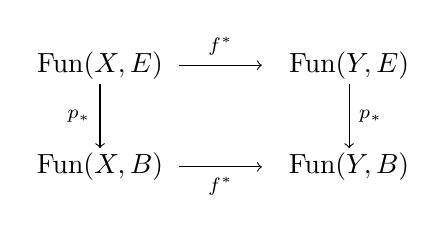
\begin{tikzpicture}[x=1.5em,y=1.5em]
  \node (FxE) at (0,1.4) {$\mathrm{Fun}(X,E)$};
  \node (FyE) at (6.0,1.4) {$\mathrm{Fun}(Y,E)$};
  \draw[->] (1.9,1.4) -- node[above]{$\scriptstyle f^{*}$} (3.9,1.4);
  \draw[->] (0,0.95) -- node[left]{$\scriptstyle p_{*}$} (0,-0.6);
  \draw[->] (6.0,0.95) -- node[right]{$\scriptstyle p_{*}$} (6.0,-0.6);
  \node (FxB) at (0,-1.05) {$\mathrm{Fun}(X,B)$};
  \node (FyB) at (6.0,-1.05) {$\mathrm{Fun}(Y,B)$};
  \draw[->] (1.9,-1.05) -- node[below]{$\scriptstyle f^{*}$} (3.9,-1.05);
\end{tikzpicture}
\end{center}
\end{enumerate}
\end{proposition}

\begin{proof}
若 $p\colon E\twoheadrightarrow B$ 是一条\trCartesianFibration，则定理 5.2.8(ii)
构造出 $i_{1}\hat{p}\colon E^{2}\to\mathrm{Hom}_{B}(B,p)$ 的一个右伴随右逆。
单纯二函子
$\mathrm{Fun}\colon\mathcal{K}^{\mathrm{op}}\times\mathcal{K}\to\mathcal{Q}\mathit{Cat}$
定义了一个 2-函子
$\mathrm{Fun}\colon\mathfrak{h}\mathcal{K}^{\mathrm{op}}\times\mathfrak{h}\mathcal{K}\to\mathfrak{h}\mathcal{Q}\mathit{Cat}$，
后者转置为一个 Yoneda 型嵌入
$\mathrm{Fun}\colon\mathfrak{h}\mathcal{K}\to\mathfrak{h}\mathcal{Q}\mathit{Cat}^{\mathfrak{h}\mathcal{K}^{\mathrm{op}}}$，
它从 $\mathcal{K}$ 的\trHomotopyTwoCategory{}出发，取值于由 2-函子、2-自然变换与%
修正组成的 2-范畴（见 B.2 节）。
这一 2-函子把伴随 $i_{1}\hat{p}\dashv\qcor{\chi}$ 送到 2-范畴
$\mathfrak{h}\mathcal{Q}\mathit{Cat}^{\mathfrak{h}\mathcal{K}^{\mathrm{op}}}$
中的一个伴随。这后一伴随对每个 $X\in\mathcal{K}$ 都定义了一个右伴随右逆伴随
\begin{center}
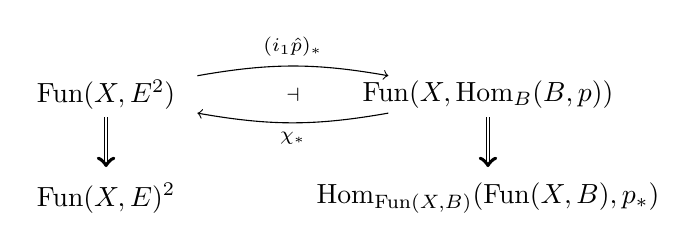
\begin{tikzpicture}[x=1.5em,y=1.5em]
  \node (FE2) at (0,2.3) {$\mathrm{Fun}(X,E^{2})$};
  \node (FH)  at (9.2,2.3) {$\mathrm{Fun}(X,\mathrm{Hom}_{B}(B,p))$};
  \draw[->] (2.2,2.75) to[bend left=10] node[above]{$\scriptstyle(i_{1}\hat{p})_{*}$} (6.8,2.75);
  \draw[->] (6.8,1.85) to[bend left=10] node[below]{$\scriptstyle\qcor{\chi}_{*}$} (2.2,1.85);
  \node at (4.5,2.3) {$\scriptstyle\dashv$};
  \draw[double,->] (0,1.75) -- (0,0.55);
  \draw[double,->] (9.2,1.75) -- (9.2,0.55);
  \node (FE2b) at (0,-0.2) {$\mathrm{Fun}(X,E)^{2}$};
  \node (Hb) at (9.2,-0.2) {$\mathrm{Hom}_{\mathrm{Fun}(X,B)}(\mathrm{Fun}(X,B),p_{*})$};
\end{tikzpicture}
\end{center}
并且对 $\mathcal{K}$ 中的每个 $f\colon Y\to X$ 定义了一个严格伴随态射，它与左、右%
伴随以及诸单位与诸余单位都严格交换：\footnote{特别地，恒同
$(i_{1}\hat{p})_{*}f^{*}=f^{*}(i_{1}\hat{p})_{*}$ 的对应是恒同
$f^{*}\qcor{\chi}_{*}=\qcor{\chi}_{*}f^{*}$。}
\begin{rveq}\label{eq:strict-adjunction-morphism}
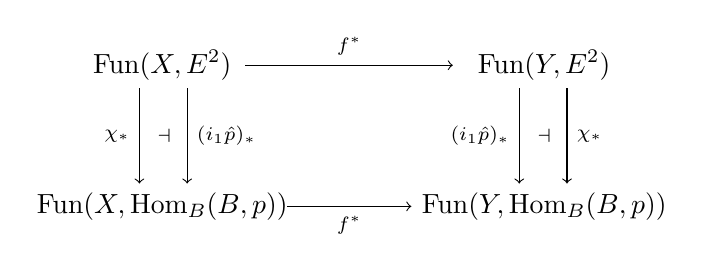
\begin{tikzpicture}[x=1.5em,y=1.5em]
  \node (TL) at (0,2.4) {$\mathrm{Fun}(X,E^{2})$};
  \node (TR) at (9.2,2.4) {$\mathrm{Fun}(Y,E^{2})$};
  \draw[->] (2.0,2.4) -- node[above]{$\scriptstyle f^{*}$} (7.0,2.4);
  \node (BL) at (0,-1.0) {$\mathrm{Fun}(X,\mathrm{Hom}_{B}(B,p))$};
  \node (BR) at (9.2,-1.0) {$\mathrm{Fun}(Y,\mathrm{Hom}_{B}(B,p))$};
  \draw[->] (3.0,-1.0) -- node[below]{$\scriptstyle f^{*}$} (6.0,-1.0);
  \draw[->] (-0.55,1.85) -- node[left]{$\scriptstyle\qcor{\chi}_{*}$} (-0.55,-0.45);
  \draw[->] (0.6,1.85) -- node[right]{$\scriptstyle(i_{1}\hat{p})_{*}$} (0.6,-0.45);
  \node at (0.05,0.7) {$\scriptstyle\dashv$};
  \draw[->] (8.6,1.85) -- node[left]{$\scriptstyle(i_{1}\hat{p})_{*}$} (8.6,-0.45);
  \draw[->] (9.75,1.85) -- node[right]{$\scriptstyle\qcor{\chi}_{*}$} (9.75,-0.45);
  \node at (9.2,0.7) {$\scriptstyle\dashv$};
\end{tikzpicture}
\end{rveq}

由定理 5.2.8(ii) 与定理 5.3.4(ii)，这就证明了陈述中的两个条件。

反之，若 $p\colon E\twoheadrightarrow B$ 满足条件 (i) 与 (ii)，则由定理
5.2.8(ii) 与定理 5.3.4(ii)，存在一个交换方块
$(i_{1}\hat{p})_{*}f^{*}=f^{*}(i_{1}\hat{p})_{*}$，其中两条竖直
$(i_{1}\hat{p})_{*}$ 都容许右伴随右逆 $(i_{1}\hat{p})_{*}\dashv\bar{r}$，而恒同
$(i_{1}\hat{p})_{*}f^{*}=f^{*}(i_{1}\hat{p})_{*}$ 的对应定义一个同构
$f^{*}\bar{r}\cong\bar{r}f^{*}$。利用诸右伴随 $\bar{r}$，我们把内部右伴随函子
$\qcor{\chi}\colon\mathrm{Hom}_{B}(B,p)\to E^{2}$ 提取为恒同元素的像
\[
\begin{gathered}
\mathrm{Fun}(\mathrm{Hom}_{B}(B,p),\mathrm{Hom}_{B}(B,p))
\;\xrightarrow{\ \ F\ \ }\;
\mathrm{Fun}(\mathrm{Hom}_{B}(B,p),E^{2})\\
\mathrm{id}\;\xmapsto{\qquad\qquad\qquad\ \ }\;\qcor{\chi}
\end{gathered}
\]
余单位可类似地内化。关于诸对应的条件用来定义单位，并验证那些表明
$i_{1}\hat{p}\dashv\qcor{\chi}$ 的\trTriangleEqualities（见命题 B.6.2）。现在%
定理 5.2.8(ii) 证明 $p\colon E\twoheadrightarrow B$ 是一条\trCartesianFibration。
\end{proof}

沿同一思路的一个更简单的论证给出：

\begin{corollary}\label{cor:cartesian-functor-representable}
\trCartesianFibration{}之间的一个交换方块，若如下左所示
\begin{center}
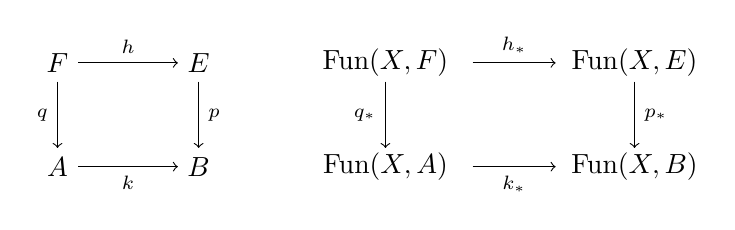
\begin{tikzpicture}[x=1.5em,y=1.5em]
  \node (F) at (0,1.5) {$F$};
  \node (E) at (3.4,1.5) {$E$};
  \node (A) at (0,-1.0) {$A$};
  \node (B) at (3.4,-1.0) {$B$};
  \draw[->] (0.5,1.5) -- node[above]{$\scriptstyle h$} (2.9,1.5);
  \draw[->] (0,1.05) -- node[left]{$\scriptstyle q$} (0,-0.55);
  \draw[->] (3.4,1.05) -- node[right]{$\scriptstyle p$} (3.4,-0.55);
  \draw[->] (0.5,-1.0) -- node[below]{$\scriptstyle k$} (2.9,-1.0);
  \node at (5.5,0.25) {$\rightsquigarrow$};
  \begin{scope}[shift={(7.9,0)}]
  \node (FxF) at (0,1.5) {$\mathrm{Fun}(X,F)$};
  \node (FxE) at (6.0,1.5) {$\mathrm{Fun}(X,E)$};
  \node (FxA) at (0,-1.0) {$\mathrm{Fun}(X,A)$};
  \node (FxB) at (6.0,-1.0) {$\mathrm{Fun}(X,B)$};
  \draw[->] (2.1,1.5) -- node[above]{$\scriptstyle h_{*}$} (4.1,1.5);
  \draw[->] (0,1.05) -- node[left]{$\scriptstyle q_{*}$} (0,-0.55);
  \draw[->] (6.0,1.05) -- node[right]{$\scriptstyle p_{*}$} (6.0,-0.55);
  \draw[->] (2.1,-1.0) -- node[below]{$\scriptstyle k_{*}$} (4.1,-1.0);
  \end{scope}
\end{tikzpicture}
\end{center}
则在\trInfinityCosmos{} $\mathcal{K}$ 中定义一个笛卡尔函子，当且仅当对所有的
$X\in\mathcal{K}$，上右所示的方块在\trQuasiCategory{}的诸\trCartesianFibration{}%
之间定义一个笛卡尔函子。
\end{corollary}

\begin{proof}
\cref{ex:prove-cartesian-functor-representable}。
\end{proof}

特别地，若 $p\colon E\twoheadrightarrow B$ 是一条\trCartesianFibration，则
$p_{*}\colon\mathrm{Fun}(X,E)\twoheadrightarrow\mathrm{Fun}(X,B)$ 亦然。下面我们
考虑 $p$-笛卡尔箭头与 $p_{*}$-笛卡尔箭头之间的关系。
\begin{lemma}\label{lem:pstar-cartesian-domain-one}
考虑\trInfinityCategory{}之间的一条\trCartesianFibration{}
$p\colon E\twoheadrightarrow B$。下左的一个 2-胞腔对
$p\colon E\twoheadrightarrow B$ 而言是\trCartesian，当且仅当与之对应的下右
2-胞腔对 $p_{*}\colon\mathrm{Fun}(X,E)\twoheadrightarrow\mathrm{Fun}(X,B)$ 而言%
是\trCartesian：
\begin{center}
\cellpair{X}{E}{e'}{e}{\psi}
\quad $\bijarrow$ \quad
\cellpair{1}{\mathrm{Fun}(X,E)}{e'}{e}{\psi}
\end{center}
\end{lemma}

左边的\trNaturalTransformation{}定义了\trHomCategory{} $\mathrm{hFun}(X,E)$ 中的%
一支箭头，而右边的\trNaturalTransformation{}则定义了\trHomCategory{}
$\mathrm{hFun}(1,\mathrm{Fun}(X,E))$ 中的一支箭头。这两个 hom-范畴是同构的，这为%
我们对其对象与箭头所作的混同记法提供了正当性。在 $E$ 中的诸 $X$-形箭头
$\qcor{\psi}\colon X\to E^{2}$ 与 $\mathrm{Fun}(X,E)$ 中的诸 1-箭头
$\qcor{\psi}\colon 1\to\mathrm{Fun}(X,E)^{2}$ 之间也有一个类似的双射对应。

\begin{proof}
由于 $p\colon E\twoheadrightarrow B$ 是一条\trCartesianFibration，上左的一支%
\trNaturalTransformation{}是 $p$-\trCartesian，当且仅当它满足命题 5.1.13 的弱%
\trUniversalProperty，而这些弱泛性质完全参照函子
$p_{*}\colon\mathrm{hFun}(X,E)\to\mathrm{hFun}(X,B)$ 来陈述。类似地，由于
$p_{*}\colon\mathrm{Fun}(X,E)\twoheadrightarrow\mathrm{Fun}(X,B)$ 是一条%
\trCartesianFibration，上右的一支\trNaturalTransformation{}是
$p_{*}$-\trCartesian，当且仅当它满足命题 5.1.13 的弱\trUniversalProperty，即完全%
参照 $p_{*}\colon\mathrm{hFun}(1,\mathrm{Fun}(X,E))\to\mathrm{hFun}(1,\mathrm{Fun}(X,B))$
来陈述。由于这些函子是同构的，$p$-笛卡尔变换与 $p_{*}$-笛卡尔变换
$\psi\colon e'\Rightarrow e$ 相重合。
\end{proof}

\cref{lem:pstar-cartesian-domain-one}刻画了定义域为 $1$ 的诸 $p_{*}$-笛卡尔变换。
更一般地：

\begin{lemma}\label{lem:pstar-cartesian-components}
下左的一支\trNaturalTransformation
\begin{center}
\cellpair{Q}{\mathrm{Fun}(X,E)}{e'}{e}{\psi}
\qquad
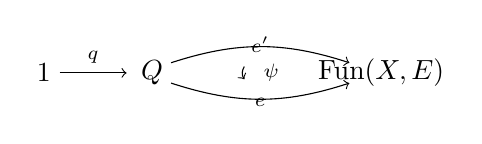
\begin{tikzpicture}[x=1.15em,y=1.15em]
  \node (o) at (0,0) {$1$};
  \node (Q)  at (3.4,0) {$Q$};
  \node (F)  at (10.6,0) {$\mathrm{Fun}(X,E)$};
  \draw[->] (0.5,0) -- node[above]{$\scriptstyle q$} (2.6,0);
  \draw[->] (4.0,0.32) to[bend left=18] (9.6,0.32);
  \node at (6.8,0.88) {$\scriptstyle e'$};
  \draw[->] (4.0,-0.32) to[bend right=18] (9.6,-0.32);
  \node at (6.8,-0.93) {$\scriptstyle e$};
  \draw[->] (6.3,0.2) to[bend right=32] (6.3,-0.2);
  \node at (7.15,0) {$\scriptstyle\psi$};
\end{tikzpicture}
\quad $\bijarrow$ \quad
\cellpair{X}{E}{e'q}{eq}{\psi q}
\end{center}
是 $p_{*}$-\trCartesian，当且仅当它的每个分量 $\psi q$ 都是 $p$-\trCartesian。
\end{lemma}

\begin{proof}
若 $\psi$ 是 $p_{*}$-\trCartesian，则由引理 5.1.4，它沿任何\trElement{}
$q\colon 1\to Q$ 的限制亦是。由\cref{lem:pstar-cartesian-domain-one}，这告诉我们
$\psi q$ 定义一条 $p$-笛卡尔变换。

反之，若 $\psi q$ 是一条 $p$-笛卡尔变换，则%
\cref{lem:pstar-cartesian-domain-one}告诉我们 $\psi q$ 是一条 $p_{*}$-笛卡尔%
变换。现在考虑穿过 $p_{*}\psi$ 的 $p_{*}$-笛卡尔提升 $\chi$ 的因子分解
$\psi=\chi\cdot\zeta$。由于 $\psi$ 的诸分量 $\psi q$ 是 $p_{*}$-\trCartesian，
$\zeta$ 的诸分量 $\zeta q$ 都是\trIsomorphism。由第 1 章中的推论 1.1.22，指数拟%
范畴 $\mathrm{Fun}(X,E)^{Q}$ 中的一支箭头是\trIsomorphism，当且仅当它是逐点同构，
故这蕴含 $\zeta$ 是一个\trIsomorphism。由笛卡尔变换的同构稳定性（见引理
5.1.6），我们于是得出结论：$\psi$ 是 $p_{*}$-\trCartesian。
\end{proof}


\subsection*{练习}

\begin{exercise}\label{ex:prove-cartesian-functor-representable}
证明\cref{cor:cartesian-functor-representable}。
\end{exercise}

